\newcommand{\coproduct}{\tikz[baseline=-0.5ex] \node[bcircle] {};}
\newcommand{\product}{\tikz[baseline=-0.5ex] \node[bsquare] {};}

\section{Correspondence between prograph rotation and involution on standard Young tableaux}

Let us recall a bijection $f$ from the set $\text{PC}(n)$ of prographs with $n$ products and $n$ coproducts to the set $\text{ST}(n^3)$ of standard Young tableaux of shape $(n,n,n)$. \cite{borie2017three} It executes through the following steps:
\begin{enumerate}
  \item Label the edges (more precisely wires, because the input to the first coproduct starts from nothing) of the prograph in depth-left first order (down-up, left-right), starting from $1$, such that output(s) of the operations are labeled after their input(s). The output of the last product is excluded.
  \item Put the numbers into the $3\times n$ Young diagram as follows: the first row contains the labels of the inputs of coproducts, the second row contains the left inputs of products, and the third row contains right inputs.
\end{enumerate}

\begin{example}
  Figure \ref{fig:prograph-young} shows a edge-labeled prograph and its corresponding standard Young tableau under the bijection $f$.
\end{example}

\begin{figure}[ht]
  \centering
  \begin{tikzpicture}[baseline=(current bounding box.center), scale=1, thick]
    \node[bcircle] (c1) at (0, 0) {};

    \node[bcircle] (c21) at (-1, 1) {};
    \coordinate (e22) at (1, 1);

    \coordinate (e31) at (-2, 2);
    \node[bsquare] (s32) at (0, 2) {};

    \coordinate (e3-5) at (-2.5, 2.5);

    \coordinate (e41) at (-2, 3);
    \node[bcircle] (c42) at (0, 3) {};

    \node[bsquare] (s51) at (-1, 4) {};
    \node[bcircle] (c52) at (1, 4) {};

    \node[bsquare] (s61) at (0, 5) {};
    \coordinate (e62) at (2, 5);

    \node[bsquare] (s71) at (1, 6) {};

    \draw (0, -0.8)
    -- node[left=0.15cm] {1} (c1);

    \draw (s71)
    -- node[left=0.15cm] {} (1, 6.8);

    \draw (c1)
    -- node[left=0.1cm] {2} (c21)
    -- node[left=0.1cm] {3} (e3-5)
    -- (s51)
    -- node[left=0.1cm] {8} (s61)
    -- node[left=0.1cm] {11} (s71);

    \draw (c1)
    -- node[right=0.1cm] {5} (e22)
    -- (s32)
    -- node[left=0.1cm] {6} (c42)
    -- node[right=0.1cm] {9} (c52)
    -- node[right=0.1cm] {12} (e62)
    -- (s71);
    \draw (c21)
    -- node[left] {4} (s32);
    \draw (c42)
    -- node[left=0.1cm] {7} (s51);
    \draw (c52)
    -- node[left=0.1cm] {10} (s61);

  \end{tikzpicture}
  \hspace{2cm}%
  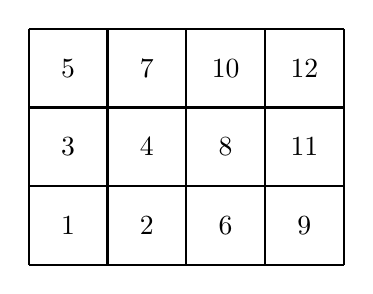
\begin{tikzpicture}[baseline=(current bounding box.center), scale=1, thick]
    \draw (0, 0) grid (4, 3);

    % Placeholders for numbers (row 1 is top)
    % Row 1 (inputs of coproducts)
    \node at (0.5, 2.5) {5}; \node at (1.5, 2.5) {7}; \node at (2.5, 2.5) {10}; \node at (3.5, 2.5) {12};
    % Row 2 (left inputs of products)
    \node at (0.5, 1.5) {3}; \node at (1.5, 1.5) {4}; \node at (2.5, 1.5) {8}; \node at (3.5, 1.5) {11};
    % Row 3 (right inputs of products)
    \node at (0.5, 0.5) {1}; \node at (1.5, 0.5) {2}; \node at (2.5, 0.5) {6}; \node at (3.5, 0.5) {9};
  \end{tikzpicture}
  \caption{An edge-labeled size-$4$ prograph and its corresponding Young tableau}
  \label{fig:prograph-young}
\end{figure}

Let $Y_k[i]$ be the $i$-th entry in the $k$-th row of the Young tableau $Y$, where $1\le i \le n$ and $1\le k \le 3$. We make simple observations: the left output of a coproduct is traversed right after its input, and the right input of a product is traversed right after its left input, as illustrated in Figure \ref{fig:edge-patterns}.

\begin{figure}[ht]
  \centering
  \begin{tikzpicture}[baseline=(current bounding box.center), scale=1, thick]
    \node[bcircle] (c1) at (0, 0) {};

    \coordinate (e21) at (-1, 1);
    \coordinate (e22) at (1, 1);

    \draw (0, -1)
    -- node[left=0.15cm] {$a$} (c1);
    \draw (c1)
    -- node[left=0.1cm] {$a+1$} (e21);
    \draw (c1)
    -- node[right=0.1cm] {$b$} (e22);

    \node at (0,-2) {$(a\in Y_1, b > a+1)$};
  \end{tikzpicture}
  \hspace{2cm}%
  \begin{tikzpicture}[baseline=(current bounding box.center), scale=1, thick]
    \node[bsquare] (c1) at (0, 0) {};

    \draw (-1, -1)
    -- node[left=0.15cm] {$a$} (c1);
    \draw (1, -1)
    -- node[right=0.15cm] {$b$} (c1);
    \draw (c1)
    -- node[right=0.1cm] {$b+1$} (0,1);

    \node at (0,-2) {$(a\in Y_2, b\in Y_3, b > a)$};
  \end{tikzpicture}
  \caption{The labeling patterns of the edges of products and coproducts}
  \label{fig:edge-patterns}.
\end{figure}

\begin{proposition}
  The map $f$ is indeed a bijection between $\text{PC}(n)$ and $\text{ST}(n^3)$.
\end{proposition}
\begin{proof}
  Firstly, we show that an image of $f$ is a Young tableau. The entries in each row are increasing by the way we put numbers into the Young diagram.

  Now we show that the entries in each column are increasing. For each each product, its right input is traversed after its left input. The number of left inputs and right inputs are the same, so we have $Y_2[i] < Y_3[i]$ for all $i$.

  During the depth-first search, traversing a left product input (Row 2) requires following an active branch. Traversing a coproduct input (Row 1) generates a new active branch. Because the DFS cannot traverse a branch that has not yet been generated, at any step $k$ in the traversal, the total number of Row 1 edges seen so far must be greater than or equal to the total number of Row 2 edges seen so far. Let the $i$-th element of Row 2 be $k$ i.e. $Y_2[i] = k$. By step $k$, the DFS has encountered exactly $i$ elements of Row 2. By the prefix inequality, the DFS must have already encountered at least $i$ elements of Row 1 by step $k$. Therefore, the $i$-th element of Row 1 must have been encountered at some step strictly prior to $k$. Thus, $Y_1[i] < Y_2[i]$.

  To have the inverse of $f$, we look at the integers in the Young tableau in increasing order. At each step, if there are available appropriate free edges, there is exactly one way to choose the left-most appropriate free edge and the next type of node to attach to it. This way coincides with the depth-left first order. So we only need to show that there are always appropriate free edges. This is true since the Young tableau always have more elements in Row 1 than in Row 2 at any prefix, and more elements in Row 2 than in Row 3 at any prefix. Before the final step $3n$, there is exactly one free edge left, which is then the right output of the last product. The constructed graph is indeed a prograph.
\end{proof}

Define the rotation $R(P)$ for a prograph $P$ by rotating it $180^\circ$ in the plane, then interchange between products and coproducts. Then $f(R(P))$ is the Schützenberger involution of $f(P)$, which can be computed rotating the Young tableau $180^\circ$ and then replacing each entry $i$ with $3n+1-i$ \cite{borie2017three}.

\begin{example}
  The prograph in Figure \ref{fig:prograph-young} and its rotation are shown in Figure \ref{fig:prograph-rotation}. The process of obtaining the Young tableau of the rotation from the original Young tableau is shown in Figure \ref{fig:young-involution}. This is clear since the traversing order of $R(P)$ is the reverse of that of $P$, and the labels are assigned in increasing order. Hence, the label $i$ in $P$ corresponds to the label $3n+1-i$ in $R(P)$.
\end{example}

\begin{figure}[ht]
  \centering
  \begin{tikzpicture}[baseline=(current bounding box.center), scale=1, thick]
    \node[bcircle] (c1) at (0, 0) {};

    \node[bcircle] (c21) at (-1, 1) {};
    \coordinate (e22) at (1, 1);

    \coordinate (e31) at (-2, 2);
    \node[bsquare] (s32) at (0, 2) {};

    \coordinate (e3-5) at (-2.5, 2.5);

    \coordinate (e41) at (-2, 3);
    \node[bcircle] (c42) at (0, 3) {};

    \node[bsquare] (s51) at (-1, 4) {};
    \node[bcircle] (c52) at (1, 4) {};

    \node[bsquare] (s61) at (0, 5) {};
    \coordinate (e62) at (2, 5);

    \node[bsquare] (s71) at (1, 6) {};

    \draw (0, -0.8)
    -- node[left=0.15cm] {1} (c1);

    \draw (s71)
    -- node[left=0.15cm] {} (1, 6.8);

    \draw (c1)
    -- node[left=0.1cm] {2} (c21)
    -- node[left=0.1cm] {3} (e3-5)
    -- (s51)
    -- node[left=0.1cm] {8} (s61)
    -- node[left=0.1cm] {11} (s71);

    \draw (c1)
    -- node[right=0.1cm] {5} (e22)
    -- (s32)
    -- node[left=0.1cm] {6} (c42)
    -- node[right=0.1cm] {9} (c52)
    -- node[right=0.1cm] {12} (e62)
    -- (s71);
    \draw (c21)
    -- node[left] {4} (s32);
    \draw (c42)
    -- node[left=0.1cm] {7} (s51);
    \draw (c52)
    -- node[left=0.1cm] {10} (s61);

  \end{tikzpicture}
  \hspace{0.5cm}
  \tikz[baseline=-0.5ex] \draw[<->, thick] (0,0) -- (2,0);
  \hspace{0.5cm}%
  \begin{tikzpicture}[baseline=(current bounding box.center), scale=1, thick]
    \node[bcircle] (c1) at (0, 0) {};

    \coordinate (e21) at (-1, 1);
    \node[bcircle] (c22) at (1, 1) {};

    \node[bsquare] (s31) at (0, 2) {};
    \node[bcircle] (c32) at (2, 2) {};

    \node[bsquare] (s41) at (1, 3) {};

    \coordinate (e4-5) at (3.5, 3.5);

    \node[bcircle] (c51) at (1, 4) {};

    \coordinate (e61) at (0, 5);
    \node[bsquare] (s62) at (2, 5) {};

    \node[bsquare] (s71) at (1, 6) {};

    \draw (0, -0.8)
    -- node[left=0.1cm] {1} (c1)
    -- node[left=0.1cm] {2} (e21)
    -- node[left=0.1cm] {} (s31)
    -- node[left=0.1cm] {5} (s41)
    -- node[left=0.1cm] {8} (c51)
    -- node[left=0.1cm] {9} (e61)
    -- node[left=0.1cm] {} (s71)
    -- (1, 6.8);

    \draw (c1)
    -- node[left=0.1cm] {3} (c22)
    -- node[left=0.1cm] {4} (s31);

    \draw (c22)
    -- node[right=0.1cm] {6} (c32)
    -- node[right=0.1cm] {7} (s41);

    \draw (c32)
    -- node[right=0.1cm] {11} (e4-5)
    -- node[right=0.1cm] {} (s62)
    -- node[right=0.1cm] {12} (s71);

    \draw (c51)
    -- node[left=0.1cm] {10} (s62);
  \end{tikzpicture}
  \caption{An edge-labeled size-$4$ prograph and its corresponding Young tableau}
  \label{fig:prograph-rotation}
\end{figure}


\begin{figure}[ht]
  \centering
  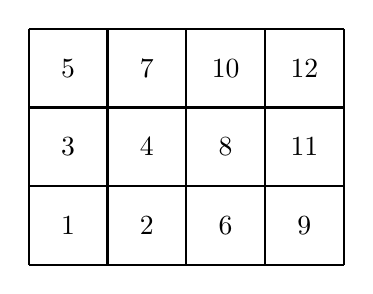
\begin{tikzpicture}[baseline=(current bounding box.center), scale=1, thick]
    \draw (0, 0) grid (4, 3);

    % Placeholders for numbers (row 1 is top)
    % Row 1 (inputs of coproducts)
    \node at (0.5, 2.5) {5}; \node at (1.5, 2.5) {7}; \node at (2.5, 2.5) {10}; \node at (3.5, 2.5) {12};
    % Row 2 (left inputs of products)
    \node at (0.5, 1.5) {3}; \node at (1.5, 1.5) {4}; \node at (2.5, 1.5) {8}; \node at (3.5, 1.5) {11};
    % Row 3 (right inputs of products)
    \node at (0.5, 0.5) {1}; \node at (1.5, 0.5) {2}; \node at (2.5, 0.5) {6}; \node at (3.5, 0.5) {9};
  \end{tikzpicture}
  \tikz[baseline=-0.5ex] \draw[->, thick] (0,0) -- node[above, font=\footnotesize] {$\substack{i\mapsto\\3n+1-i}$} (1.5,0);
  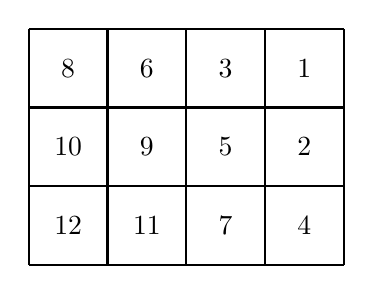
\begin{tikzpicture}[baseline=(current bounding box.center), scale=1, thick]
    \draw (0, 0) grid (4, 3);

    \node at (0.5, 2.5) {8}; \node at (1.5, 2.5) {6}; \node at (2.5, 2.5) {3}; \node at (3.5, 2.5) {1};

    \node at (0.5, 1.5) {10}; \node at (1.5, 1.5) {9}; \node at (2.5, 1.5) {5}; \node at (3.5, 1.5) {2};

    \node at (0.5, 0.5) {12}; \node at (1.5, 0.5) {11}; \node at (2.5, 0.5) {7}; \node at (3.5, 0.5) {4};
  \end{tikzpicture}
  \tikz[baseline=-0.5ex] \draw[->, thick] (0,0) -- node[above, font=\footnotesize] {rotate} (1.5,0);
  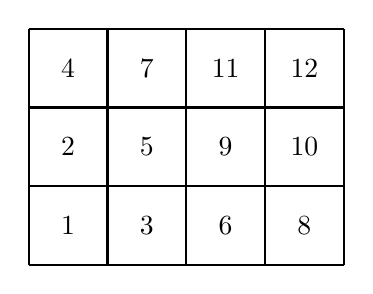
\begin{tikzpicture}[baseline=(current bounding box.center), scale=1, thick]
    \draw (0, 0) grid (4, 3);

    % Placeholders for numbers (row 1 is top)
    % Row 1 (inputs of coproducts)
    \node at (0.5, 2.5) {4}; \node at (1.5, 2.5) {7}; \node at (2.5, 2.5) {11}; \node at (3.5, 2.5) {12};
    % Row 2 (left inputs of products)
    \node at (0.5, 1.5) {2}; \node at (1.5, 1.5) {5}; \node at (2.5, 1.5) {9}; \node at (3.5, 1.5) {10};
    % Row 3 (right inputs of products)
    \node at (0.5, 0.5) {1}; \node at (1.5, 0.5) {3}; \node at (2.5, 0.5) {6}; \node at (3.5, 0.5) {8};
  \end{tikzpicture}
  \caption{Schützenberger involution of the Young tableau in Figure \ref{fig:prograph-young}.}
  \label{fig:young-involution}
\end{figure}


\section{Diameter notion for prographs and its computation from the corresponding standard Young tableaux}

It is natural to inherit the notion of diameter from general graph theory, that is the maximum distance between any two vertices in the graph. It is left to define the distance between two vertices. A precise definition is shown below.

\begin{definition}
  Let $P=(V,E)$ be a prograph, for $u,v\in V$, we define the distance $d(u,v)$ to be the length of the longest path between them, where $d(u,v)=\infty$ if no such path exists. The diameter of $P$ is defined as
  $$d_P = \max_{u,v \in V} \left\{d(u,v) : u,v \in V \text{ and } d(u,v) < \infty\right\}.$$
\end{definition}

Let $c_1$ be the first coproduct and $p_n$ be the last product. The diameter $d_P$ is exactly $d(c_1,p_n)$. This perfectly matches the notion of \textit{maximal chain} in posets.

We describe how to compute $d_P$ from the corresponding Young tableau. Let $L[i], 1\le i\le 3n+1$ be the length of the longest path from $c_1$ to the node that the edge labeled $i$ is an input to. For the last output, it is the input to the node at infinity. We have $L[1]=0$ and $d_P = L[3n+1]-1$. We use the results in the next section when the labels of the edges are computed from the Young tableau.

\begin{itemize}
  \item For each coproduct $c_i$, $(1\le i\le n)$, we have the corresponding tuple $(in, out_L, out_R)$. Then
        $$L[out_L] = L[out_R] = L[in]+1.$$
  \item For each product $p_i (1\le i\le n)$, we have the corresponding tuple $(in_L, in_R, out)$. Then
        $$L[out] = \max\{L[in_L], L[in_R]\} + 1.$$
\end{itemize}

\begin{example}
  Take the Young tableau in Figure \ref{fig:prograph-young}. We order the nodes together with their tuples as follows.
  \begin{table}[ht]
    \begin{center}
      \begin{tabular*}{0.5\textwidth}{@{\extracolsep{\fill}}ccc}
        $i$-th node & Type & Tuple       \\
        \hline
        1           & \coproduct  & $(1, 2, 5)$ \\
        2           & \coproduct  & $(2, 3, 4)$ \\
        3           & \product     & $(4, 5, 6)$ \\
        4           & \coproduct  & $(6, 7, 9)$ \\
        5           & \product     & $(3, 7, 8)$\\
        6           & \coproduct  & $(9, 10, 12)$ \\
        7           & \product     & $(8, 10, 11)$ \\
        8           & \product     & $(11, 12, 13)$
      \end{tabular*}
    \end{center}
    \caption{The order of the nodes and their tuples for the prograph in Figure \ref{fig:prograph-young}.}
    \label{tab:node-tuples}
  \end{table}


  We can compute $L[i]$ for $1\le i \le 12$ as follows in one pass.
  \begin{itemize}
    \item $L[1] = 0$;
    \item $L[2] = L[5] = L[1]+1 = 1$;
    \item $L[3] = L[4] = L[2]+1 = 2$;
    \item $L[6] = \max\{L[4], L[5]\} + 1 = 3$;
    \item $L[7] = L[9] = L[6]+1 = 4$;
    \item $L[8] = \max\{L[3], L[7]\} + 1 = 5$;
    \item $L[10] = L[12] = L[9]+1 = 5$;
    \item $L[11] = \max\{L[8], L[10]\} + 1 = 6$;
    \item $L[13] = \max\{L[11], L[12]\} + 1 = 7$.
  \end{itemize}
  Hence, $d_P = L[13] - 1 = 6$.
\end{example}

\section{Computation of labels of coproduct outputs and product inputs from Young tableaux}

Let the products and coproducts be ordered by their topological order i.e. when their input(s) have been traversed in depth-left first order \cite{borie2017three}.

\begin{example}
  The order of the nodes in the prograph in Figure \ref{fig:prograph-young} is shown in Figure \ref{fig:prograph-order}.
\end{example}

\begin{figure}[ht]
  \centering
  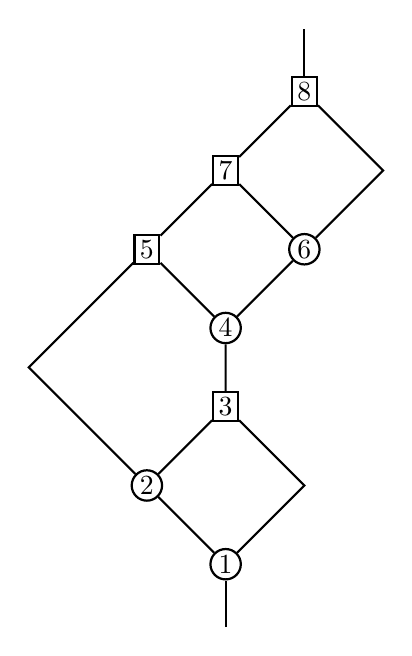
\begin{tikzpicture}[baseline=(current bounding box.center), scale=1, thick]
    \node[circle, draw, inner sep=1pt] (c1) at (0, 0) {1};

    \node[circle, draw, inner sep=1pt] (c21) at (-1, 1) {2};
    \coordinate (e22) at (1, 1);

    \coordinate (e31) at (-2, 2);
    \node[rectangle, draw, inner sep=2pt] (s32) at (0, 2) {3};

    \coordinate (e3-5) at (-2.5, 2.5);

    \coordinate (e41) at (-2, 3);
    \node[circle, draw, inner sep=1pt] (c42) at (0, 3) {4};

    \node[rectangle, draw, inner sep=2pt] (s51) at (-1, 4) {5};
    \node[circle, draw, inner sep=1pt] (c52) at (1, 4) {6};

    \node[rectangle, draw, inner sep=2pt] (s61) at (0, 5) {7};
    \coordinate (e62) at (2, 5);

    \node[rectangle, draw, inner sep=2pt] (s71) at (1, 6) {8};

    \draw (0, -0.8)
    -- (c1);

    \draw (s71)
    --(1, 6.8);

    \draw (c1)
    -- (c21)
    -- (e3-5)
    -- (s51)
    -- (s61)
    -- (s71);

    \draw (c1)
    -- (e22)
    -- (s32)
    -- (c42)
    -- (c52)
    -- (e62)
    -- (s71);
    \draw (c21)
    --  (s32);
    \draw (c42)
    -- (s51);
    \draw (c52)
    -- (s61);

  \end{tikzpicture}\hspace{2cm}%
  \caption{The order of the nodes in the prograph in Figure \ref{fig:prograph-young}}
  \label{fig:prograph-order}
\end{figure}

Using the Young tableau, we attempt to determine the node order and the labels of their outputs.

\subsection{Node order from Young tableaux}
The first row marks the steps where the input to coproducts are traversed and the third row marks the steps where the inputs to products are traversed. The order of the nodes can be determined by the relative order of these steps.

\begin{example}
  Using at the first and third rows in the Young tableau in Figure \ref{fig:prograph-young}, we derive the order of the nodes as shown in Table \ref{tab:prograph-order}.
\end{example}

\begin{table}[ht]
  \begin{center}
    \begin{tabular*}{0.8\textwidth}{@{\extracolsep{\fill}}ccccccccc}
      Number & 1 & 3 & 4 & 6 & 7 & 8 & 11 & 12 \\
      \hline
      Row & 1 & 1 & 3 & 1 & 3 & 1 & 3 & 3\\
      \hline
      Node type & \coproduct & \coproduct & \product & \coproduct & \product & \coproduct & \product & \product

    \end{tabular*}
  \end{center}
  \caption{The order of the nodes derived from the first and third rows of the Young tableau in Figure \ref{fig:prograph-young}.}
  \label{tab:prograph-order}
\end{table}


\subsection{Edge labels from Young tableaux}
For products, the right input is traversed only if the branch generated by the ascending node of its left input has been fully traversed. Hence, we assign the numbers in the second and third rows of the Young tableau to the left and right inputs of products analogously to a bracketing system.

\begin{example}
  For the Young tableau in Figure \ref{fig:prograph-young}, we have the following bracketing system for the left and right inputs of products and the corresponding left and right inputs of products as in Tables \ref{tab:product-bracket} and \ref{tab:product-inputs}.
\end{example}

\begin{table}[ht]
  \begin{center}
    \begin{tabular*}{0.8\textwidth}{@{\extracolsep{\fill}}ccccccccc}
      Number & 3 & 4 & 5 & 7 & 8 & 10 & 11 & 12 \\
      \hline
      Row & 2 & 2 & 3 & 3 & 2 & 3 & 2 & 3 \\
      \hline
      Bracket & ( & ( & ) & ) & ( & ) & ( & )\\

    \end{tabular*}
  \end{center}

  \caption{The bracketing system for the left and right inputs of products in Figure \ref{fig:prograph-young}.}
  \label{tab:product-bracket}
\end{table}

\begin{table}[ht]
  \begin{center}
    \begin{tabular*}{0.8\textwidth}{@{\extracolsep{\fill}}ccccc}
      $i$-th product & 1 & 2 & 3 & 4 \\
      \hline
      Left input & 4 & 3 & 8 & 11 \\
      \hline
      Right input & 5 & 7 & 10 & 12 \\

    \end{tabular*}
  \end{center}
  \caption{The left and right inputs of products derived from Table \ref{tab:product-bracket}.}
  \label{tab:product-inputs}
\end{table}

For coproducts,
\begin{itemize}
  \item the left output is traversed \textit{right after} the input (taken in the first row), and
  \item the right output is traversed \textit{right after} the left branch reaches a product as a left input.
\end{itemize}
Hence we can still use a bracketing system, but for the first and second rows, and adding \textit{one} the result.

\begin{example}
  For the Young tableau in Figure \ref{fig:prograph-young}, we have the following bracketing system for the inputs and outputs of coproducts and the corresponding left and right outputs of coproducts as in Tables \ref{tab:coproduct-bracket} and \ref{tab:coproduct-outputs}.
\end{example}

\begin{table}[ht]
  \begin{center}
    \begin{tabular*}{0.8\textwidth}{@{\extracolsep{\fill}}ccccccccc}
      Number & 1 & 2 & 3 & 4 & 6 & 8 & 9 & 11 \\
      \hline
      Row & 1 & 1 & 2 & 2 & 1 & 2 & 1 & 2 \\
      \hline
      Bracket & ( & ( & ) & ) & ( & ) & ( & )\\

    \end{tabular*}
  \end{center}
  \caption{The bracketing system for the inputs and outputs of coproducts in Figure \ref{fig:prograph-young}.}
  \label{tab:coproduct-bracket}
\end{table}

\begin{table}[ht]
  \begin{center}
    \begin{tabular*}{0.8\textwidth}{@{\extracolsep{\fill}}ccccc}
      $i$-th coproduct & 1 & 2 & 3 & 4 \\
      \hline
      Left input & 2+1=3 & 1+1=2 & 6+1=7 & 9+1=10 \\
      \hline
      Right input & 3+1=4 & 4+1=5 & 8+1=9 & 11+1=12 \\

    \end{tabular*}
  \end{center}
  \caption{The left and right outputs of coproducts derived from Table \ref{tab:coproduct-bracket}.}
  \label{tab:coproduct-outputs}
\end{table}

We need the following definitions for the next section.
\begin{definition}
  For each $x\in Y_1$, let $m_c(x)$ be the edge that closes the bracket that opens at $x$.

  For each $y\in Y_2$, let $m_p(y)$ be the edge that closes the bracket that opens at $y$.
\end{definition}

\begin{example}
  Take the Young tableau in Figure \ref{fig:prograph-young}. We have $m_c(2)=3, m_c(1)=4, m_c(6)=8, m_c(9)=11$ and $m_p(3)=7, m_p(4)=5, m_p(8)=10, m_p(11)=12$.
\end{example}

\section{Description of the faces of prographs when seen as Voronoi diagrams}

Let us exclude the input to the first coproduct and the output of the last product, and look at the remaining edges as a planar graph. By Euler formula for planar graphs, we have $V-E+F=2$. With $V=2n$ and $E=3n-1$, we have $F=n+1$. Hence, there are $n$ bounded faces and one unbounded face. Consider the boundary of each bounded face. The edge with the least label on the boundary must be a left output of a coproduct, and the edge with the greatest label on the boundary must be a right input of a product. Therefore, it is natural to label assign to each face a pair of coproduct-product. In particular, we assign to each face the input to its first coproduct and the output of its last product (in the DFS order). Then, using the results in the previous section, we can recover the boundary edges.

Now it is clear that from an coproduct input, we can compute the left product output that matches it using the $m_c$ function, and from a left product input, we can compute the right product output that matches it using the $m_p$ function.

\begin{example}
  For the Young tableau in Figure \ref{fig:prograph-young}, we have the following pairs of coproduct-product for each face and the corresponding boundary edges as in Table \ref{tab:face-boundary}.
\end{example}

\begin{table}[ht]
  \begin{center}
    \begin{tabular*}{0.8\textwidth}{@{\extracolsep{\fill}}ccccc}
      $i$-th face & 1 & 2 & 3 & 4 \\
      \hline
      Coproduct input $x$ & 1 & 2 & 6 & 9 \\
      $m_c(x)$ & 4 & 3 & 8 & 11 \\
      $m_p(m_c(x))$ & 5 & 7 & 10 & 12 \\
      Start coproduct tuple & $(1,2,5)$ & $(2,3,4)$ & $(6,7,9)$ & $(9,11,12)$ \\
      End product tuple & $(4,5,6)$ & $(3,7,8)$ & $(8,10,11)$ & $(11,12,13)$ \\
    \end{tabular*}
  \end{center}
  \caption{The pairs of coproduct-product tuples for each face.}
  \label{tab:face-boundary}
\end{table}

To recover the boundary edges, we recover the left and right sides of the boundary. Each includes edges selected from a path from the start coproduct to the end product. The rules are as follows.

\begin{itemize}
  \item For the left side, we start from the left output of the start coproduct. If we reach a product, simply take the output to continue. If we reach a coproduct, take the \textit{right output} to continue (otherwise we enter another face). We stop when we reach the end product.
  \item For the right side, we start from the right output of the start coproduct. If we reach a product, simply take the output to continue. If we reach a coproduct, take the \textit{left input} to continue (otherwise we enter another face). We stop when we reach the end product.
\end{itemize}

\begin{example}
  Take the first face in Table \ref{tab:face-boundary}. The path of the left side reads
  $$(1,2,5)\rightarrow (2,3,4) \rightarrow (4,5,6),$$
  from which we take edges $2$ and $4$. The path of the right side reads
  $$(1,2,5) \rightarrow (4,5,6),$$
  from which we take edge $5$. Hence, the boundary edges of the first face are $\{2,4,5\}$.
\end{example}

\section{Reasons left and right coproduct inputs are not flippable}

There are two reasons for this. Combinatorially, this would break the condition of the Young tableau that the number of Row 2 elements is always greater than or equal to the number of Row 3 elements at any prefix in the Young tableau. Geometrically, this would break the planarity of the graph.

These are also the reasons that left and right product outputs are not flippable, by considering the rotation of the prograph and the Schützenberger involution of the Young tableau.

\section{The evolution of the Young tableau when rerooting the prograph}

In this section, for a prograph, we connect the output of the last product to the input of the first coproduct, and embed it onto the sphere \cite{borie2022product}. Firstly, notice that we may only reroot the prograph at an edge between a product and a coproduct.

\begin{definition}
  Let $P$ be a prograph. The reroot operation at the edge $e$ between a product and a coproduct, if possible, is the operation that
  \begin{enumerate}
    \item orients $e$ from the product to the coproduct, and
    \item orients all the other edges in such a way that satisfies the constraints for products and coproducts in a unique way, and
    \item the resulting graph is a prograph.
  \end{enumerate}
\end{definition}

We study the cases when $n=2$, as show in Figure \ref{fig:prographs-n2} by hand to point out problems regarding rerooting

\begin{enumerate}
  \item The graph cannot be rerooted because it violates constraints for products and coproducts.
  \item The rerooted graph can not be traversed in DFS. In other words, it is non of the other prographs of the same size.
\end{enumerate}

These lead to open questions regarding counting rerootable prographs for each $n$, counting rerootable edges for each prograph, and characterizing rerootable edges.

\begin{figure}[ht]
  \centering
  \begin{subfigure}[t]{0.3\textwidth}
    \centering
    \begin{tikzpicture}[baseline=(current bounding box.center), scale=0.6, thick]
      \node[bcircle] (c1) at (0, 0) {};

      \coordinate  (e21) at (-1, 1);
      \coordinate (e22) at (1, 1);

      \node[bsquare] (s31) at (0, 2) {};

      \node[bcircle] (c41) at (0, 4) {};

      \coordinate  (e51) at (-1, 5);
      \coordinate  (e52) at (1, 5);

      \node[bsquare] (s61) at (0, 6) {};

      \draw (0, -0.8)
      edge[->, dashed] (c1);

      \draw (s61)
      edge[dashed] (0, 6.8);

      \draw[dashed] (0, 6.8) to[out=0, in=0, looseness=1] node[right] {1} (0, -0.8);

      \draw (c1) -- node[left=0.1cm] {2} (e21);
      \draw[->] (e21) -- (s31);
      \draw[->] (s31) -- node[left=0.1cm] {4} (c41);
      \draw (c41) -- node[left=0.1cm] {5} (e51);
      \draw[->] (e51) -- (s61);

      \draw (c1) -- node[right=0.1cm] {3} (e22);
      \draw[->] (e22) -- (s31);

      \draw (c41) -- node[right=0.1cm] {6} (e52);
      \draw[->] (e52) -- (s61);
    \end{tikzpicture}
    \caption{$P_1$}
  \end{subfigure}\hfill
  \begin{subfigure}[t]{0.3\textwidth}
    \centering
    \begin{tikzpicture}[baseline=(current bounding box.center), scale=0.6, thick]
      \node[bcircle] (c1) at (0, 0) {};

      \coordinate  (e21) at (-2, 2);
      \node[bcircle] (c22) at (2, 2) {};

      \node[bsquare] (s31) at (0, 4) {};
      \coordinate  (e32) at (4, 4);

      \node[bsquare] (s41) at (2, 6) {};

      \draw (0, -0.8) edge[->, dashed] (c1);
      \draw (2, 6.8) edge[dashed] (2, 6);
      \draw[dashed] (2, 6.8) to[out=0, in=0, looseness=1.5] node[right] {1} (0, -0.8);

      \draw (c1) -- node[left=0.1cm] {2} (e21);
      \draw[->] (e21) -- (s31);
      \draw (c1) edge[->] node[right=0.1cm] {3} (c22);
      \draw[->] (c22) -- node[left=0.1cm] {4} (s31);
      \draw[->] (s31) -- node[left=0.1cm] {5} (s41);
      \draw (c22) -- node[right=0.1cm] {6} (e32);
      \draw[->] (e32) -- (s41);
    \end{tikzpicture}
    \caption{$P_2$}
  \end{subfigure}\hfill
  \begin{subfigure}[t]{0.3\textwidth}
    \centering
    \begin{tikzpicture}[baseline=(current bounding box.center), scale=0.6, thick]
      \node[bcircle] (c1) at (0, 0) {};

      \node[bcircle] (c21) at (-2, 2) {};
      \coordinate  (e22) at (2, 2);

      \coordinate (e2-51) at (-3, 3);
      \coordinate (e2-52) at (-1, 3);
      \coordinate (e2-53) at (3, 3);

      \node[bsquare] (s31) at (-2, 4) {};

      \node[bsquare] (s41) at (0, 6) {};

      \draw (0, -0.8) edge[->, dashed] (c1);
      \draw (0, 6.8) edge[dashed] (0, 6);
      \draw[dashed] (0, 6.8) to[out=0, in=0, looseness=1.5] node[right] {1} (0, -0.8);

      \draw (c1) edge[->] node[left=0.1cm] {2} (c21);
      \draw (c21) -- node[left=0.1cm] {3} (e2-51)
      (e2-51) edge[->] (s31);
      \draw (c21) -- node[right=0.1cm] {4} (e2-52)
      (e2-52) edge[->] (s31);
      \draw (c1) -- node[right=0.1cm] {6} (e2-53)
      (e2-53) edge[->] (s41);
      \draw (s31) edge[->] node[left=0.1cm] {5} (s41);
    \end{tikzpicture}
    \caption{$P_3$}
  \end{subfigure}

  \vspace{1cm}

  \hspace*{0.3\textwidth}\hfill
  \begin{subfigure}[t]{0.3\textwidth}
    \centering
    \begin{tikzpicture}[baseline=(current bounding box.center), scale=0.6, thick]
      \node[bcircle] (c1) at (0, 0) {};

      \coordinate  (e21) at (2, 2);
      \node[bcircle] (c22) at (-2, 2) {};

      \node[bsquare] (s31) at (0, 4) {};
      \coordinate  (e32) at (-4, 4);

      \node[bsquare] (s41) at (-2, 6) {};

      \draw (0, -0.8) edge[->, dashed] (c1);
      \draw (-2, 6.8) edge[dashed] (-2, 6);
      \draw[dashed] (-2, 6.8) to[out=0, in=0, looseness=1.5] node[right] {1} (0, -0.8);

      \draw (c1) -- node[right=0.1cm] {5} (e21);
      \draw[->] (e21) -- (s31);
      \draw (c1) edge[->] node[left=0.1cm] {2} (c22);
      \draw[->] (c22) -- node[right=0.1cm] {4} (s31);
      \draw[->] (s31) -- node[right=0.1cm] {6} (s41);
      \draw (c22) -- node[left=0.1cm] {3} (e32);
      \draw[->] (e32) -- (s41);
    \end{tikzpicture}
    \caption{$P_2'$}
  \end{subfigure}\hfill
  \begin{subfigure}[t]{0.3\textwidth}
    \centering
    \begin{tikzpicture}[baseline=(current bounding box.center), scale=0.6, thick]
      \node[bcircle] (c1) at (0, 0) {};

      \node[bcircle] (c21) at (2, 2) {};
      \coordinate  (e22) at (-2, 2);

      \coordinate (e2-51) at (3, 3);
      \coordinate (e2-52) at (1, 3);
      \coordinate (e2-53) at (-3, 3);

      \node[bsquare] (s31) at (2, 4) {};

      \node[bsquare] (s41) at (0, 6) {};

      \draw (0, -0.8) edge[->, dashed] (c1);
      \draw (0, 6.8) edge[dashed] (0, 6);
      \draw[dashed] (0, 6.8) to[out=0, in=0, looseness=1.5] node[right] {1} (0, -0.8);

      \draw (c1) -- node[right=0.1cm] {3} (c21);
      \draw (c21) -- node[left] {5} (e2-51)
      (e2-51) edge[->] (s31);
      \draw (c21) -- node[left=0.1cm] {4} (e2-52)
      (e2-52) edge[->] (s31);
      \draw (c1) -- node[left=0.1cm] {2} (e2-53)
      (e2-53) edge[->] (s41);
      \draw (s31) edge[->] node[right=0.1cm] {6} (s41);
    \end{tikzpicture}
    \caption{$P_3'$}
  \end{subfigure}
  \caption{The five size-$2$ prographs}
  \label{fig:prographs-n2}
\end{figure}

For the graph $P_1$, we can only reroot at edge $4$ to get the same prograph (hence the same Young tableau) and cannot reroot at edge $2$ and edge $3$ as illustrated in Figure \ref{fig:rerooting-P1}. The fact that we cannot reroot at edge $5$ and $6$ is symmetric to the cases of edge $2$ and edge $3$, respectively.

\begin{figure}[ht]
  \centering
  \begin{subfigure}[t]{0.3\textwidth}
    \centering
    \begin{tikzpicture}[baseline=(current bounding box.center), scale=0.6, thick]
      \node[bcircle] (c1) at (0, 0) {};

      \coordinate  (e21) at (-1, 1);
      \coordinate (e22) at (1, 1);

      \node[bsquare] (s31) at (0, 2) {};

      \node[bcircle] (c41) at (0, 4) {};

      \coordinate  (e51) at (-1, 5);
      \coordinate  (e52) at (1, 5);

      \node[bsquare, fill=red!50] (s61) at (0, 6) {};

      \draw (0, -0.8)
      -- (c1);

      \draw (s61)
      edge[<-] (0, 6.8);

      \draw[-] (0, 6.8) to[out=0, in=0, looseness=1.5] node[right] {} (0, -0.8);

      \draw[<-, dashed] (c1) -- node[left=0.1cm] {} (e21);
      \draw[dashed] (e21) -- (s31);
      \draw[->] (s31) -- node[left=0.1cm] {} (c41);
      \draw (c41) -- node[left=0.1cm] {} (e51);
      \draw[->] (e51) -- (s61);

      \draw (c1)
      -- node[right, right=0.1cm] {} (e22)
      (e22) edge[->]  (s31);

      \draw (c41) -- node[right, right=0.1cm] {} (e52)
      (e52) edge[->] (s61);
    \end{tikzpicture}
    \caption{Rerooting at edge 2 is not possible, due to a violation at the top coproduct}
  \end{subfigure}
  \hfill
  \begin{subfigure}[t]{0.3\textwidth}
    \centering
    \begin{tikzpicture}[baseline=(current bounding box.center), scale=0.6, thick]
      \node[bcircle] (c1) at (0, 0) {};

      \coordinate  (e21) at (-1, 1);
      \coordinate (e22) at (1, 1);

      \node[bsquare] (s31) at (0, 2) {};

      \node[bcircle] (c41) at (0, 4) {};

      \coordinate  (e51) at (-1, 5);
      \coordinate  (e52) at (1, 5);

      \node[bsquare] (s61) at (0, 6) {};

      \draw (0, -0.8)
      -- (c1);

      \draw (s61)
      edge[<-] (0, 6.8);

      \draw[-] (0, 6.8) to[out=0, in=0, looseness=1.5] node[right] {} (0, -0.8);

      \draw[] (c1) -- node[left=0.1cm] {} (e21);
      \draw[->] (e21) -- (s31);
      \draw[<-] (s31) -- node[left=0.1cm] {} (c41);
      \draw (c41) -- node[left=0.1cm] {} (e51);
      \draw[->] (e51) -- (s61);

      \draw (c1)
      edge[<-, dashed] node[right, right=0.1cm] {} (e22)
      (e22) edge[dashed]  (s31);

      \draw (c41) edge[<-] node[right, right=0.1cm] {} (e52)
      (e52) edge[-] (s61);
    \end{tikzpicture}
    \caption{Rerooting at edge $3$ is not possible, since there is a bounded cycle. Note: edges $5$ and $6$ can be flipped}
  \end{subfigure}
  \hfill
  \begin{subfigure}[t]{0.3\textwidth}
    \centering
    \begin{tikzpicture}[baseline=(current bounding box.center), scale=0.6, thick]
      \node[bcircle] (c1) at (0, 0) {};

      \coordinate  (e21) at (-1, 1);
      \coordinate (e22) at (1, 1);

      \node[bsquare] (s31) at (0, 2) {};

      \node[bcircle] (c41) at (0, 4) {};

      \coordinate  (e51) at (-1, 5);
      \coordinate  (e52) at (1, 5);

      \node[bsquare] (s61) at (0, 6) {};

      \draw (0, -0.8)
      edge[->] (c1);

      \draw (s61)
      edge[] (0, 6.8);

      \draw[] (0, 6.8) to[out=0, in=0, looseness=1.5] node[right] {4} (0, -0.8);

      \draw (c1) -- node[left=0.1cm] {5} (e21);
      \draw[->] (e21) -- (s31);
      \draw[->] (s31) edge[dashed] node[left=0.1cm] {1} (c41);
      \draw (c41) -- node[left=0.1cm] {2} (e51);
      \draw[->] (e51) -- (s61);

      \draw (c1) -- node[right=0.1cm] {6} (e22);
      \draw[->] (e22) -- (s31);

      \draw (c41) -- node[right=0.1cm] {3} (e52);
      \draw[->] (e52) -- (s61);
    \end{tikzpicture}
    \caption{Rerooting at edge 4 is possible, resulting in the same prograph when relabeling the edges.}
  \end{subfigure}
  \caption{Rerooting attempts for $P_1$}
  \label{fig:rerooting-P1}
\end{figure}

For other prographs, let us only show the rerootable cases, together with the resulting corresponding Young tableau. For $P_2$, there are three rerootable edges, as shown in Figure \ref{fig:rerooting-P2}. For $P_3$, there is only one rerootable edge, as shown in Figure \ref{fig:rerooting-P3}.

\begin{figure}[ht]
  \begin{subfigure}[t]{0.45\textwidth}
    \centering
    \begin{tikzpicture}[baseline=(current bounding box.center), scale=0.55, thick]
      \node[bcircle] (c1) at (0, 0) {};

      \coordinate  (e21) at (-2, 2);
      \node[bcircle] (c22) at (2, 2) {};

      \node[bsquare] (s31) at (0, 4) {};
      \coordinate  (e32) at (4, 4);

      \node[bsquare] (s41) at (2, 6) {};

      \draw (0, -0.8) edge[] (c1);
      \draw (2, 6.8) edge[->] (s41);
      \draw[] (2, 6.8) to[out=0, in=0, looseness=1.5] node[right] {5} (0, -0.8);

      \draw (c1) edge[<-, dashed] node[left=0.1cm] {1} (e21);
      \draw (e21) edge[dashed] (s31);
      \draw (c1) edge[->] node[right=0.1cm] {2} (c22);
      \draw[->] (c22) -- node[left=0.1cm] {3} (s31);
      \draw[<-] (s31) -- node[left=0.1cm] {6} (s41);
      \draw (c22) -- node[right=0.1cm] {4} (e32);
      \draw[->] (e32) -- (s41);
    \end{tikzpicture}
    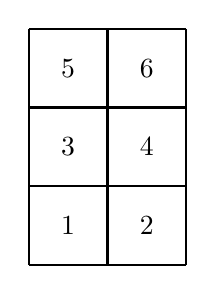
\begin{tikzpicture}[baseline=(current bounding box.center), scale=1, thick]
      \draw (0, 0) grid (2, 3);

      % Row 3
      \node at (0.5, 2.5) {5}; \node at (1.5, 2.5) {6};
      % Row 2 
      \node at (0.5, 1.5) {3}; \node at (1.5, 1.5) {4};
      % Row 1 
      \node at (0.5, 0.5) {1}; \node at (1.5, 0.5) {2};
    \end{tikzpicture}
    \caption{Rerooting at edge $2$, then relabeling}
  \end{subfigure}
  \hfill
  \begin{subfigure}[t]{0.45\textwidth}
    \centering
    \begin{tikzpicture}[baseline=(current bounding box.center), scale=0.55, thick]
      \node[bcircle] (c1) at (0, 0) {};

      \coordinate  (e21) at (-2, 2);
      \node[bcircle] (c22) at (2, 2) {};

      \node[bsquare] (s31) at (0, 4) {};
      \coordinate  (e32) at (4, 4);

      \node[bsquare] (s41) at (2, 6) {};

      \draw (0, -0.8) edge[] (c1);
      \draw (2, 6.8) edge[->] (s41);
      \draw[] (2, 6.8) to[out=0, in=0, looseness=1.5] node[right] {4} (0, -0.8);

      \draw (c1) edge[<-] node[left=0.1cm] {6} (e21);
      \draw (e21) edge[] (s31);
      \draw (c1) edge[<-] node[right=0.1cm] {3} (c22);
      \draw[<-, dashed] (c22) -- node[left=0.1cm] {1} (s31);
      \draw[<-] (s31) -- node[left=0.1cm] {5} (s41);
      \draw (c22) -- node[right=0.1cm] {2} (e32);
      \draw[->] (e32) -- (s41);
    \end{tikzpicture}
    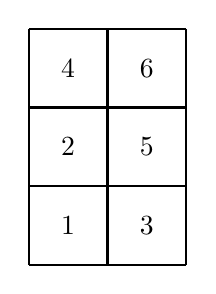
\begin{tikzpicture}[baseline=(current bounding box.center), scale=1, thick]
      \draw (0, 0) grid (2, 3);

      % Row 3
      \node at (0.5, 2.5) {4}; \node at (1.5, 2.5) {6};
      % Row 2 
      \node at (0.5, 1.5) {2}; \node at (1.5, 1.5) {5};
      % Row 1 
      \node at (0.5, 0.5) {1}; \node at (1.5, 0.5) {3};
    \end{tikzpicture}
    \caption{Rerooting at edge $4$, then relabeling}
  \end{subfigure}
  \vspace{1cm}
  \centering
  \begin{subfigure}[t]{0.45\textwidth}
    \centering
    \begin{tikzpicture}[baseline=(current bounding box.center), scale=0.55, thick]
      \node[bcircle] (c1) at (0, 0) {};

      \coordinate  (e21) at (-2, 2);
      \node[bcircle] (c22) at (2, 2) {};

      \node[bsquare] (s31) at (0, 4) {};
      \coordinate  (e32) at (4, 4);

      \node[bsquare] (s41) at (2, 6) {};

      \draw (0, -0.8) edge[] (c1);
      \draw (2, 6.8) edge[->] (s41);
      \draw[] (2, 6.8) to[out=0, in=0, looseness=1.5] node[right] {3} (0, -0.8);

      \draw (c1) edge[-] node[left=0.1cm] {4} (e21);
      \draw (e21) edge[->] (s31);
      \draw (c1) edge[<-] node[right=0.1cm] {2} (c22);
      \draw[->] (c22) -- node[left=0.1cm] {5} (s31);
      \draw[->] (s31) -- node[left=0.1cm] {6} (s41);
      \draw (c22) edge[<-, dashed] node[right=0.1cm] {1} (e32);
      \draw[dashed] (e32) -- (s41);
    \end{tikzpicture}
    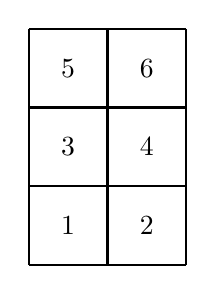
\begin{tikzpicture}[baseline=(current bounding box.center), scale=1, thick]
      \draw (0, 0) grid (2, 3);

      % Row 3
      \node at (0.5, 2.5) {5}; \node at (1.5, 2.5) {6};
      % Row 2 
      \node at (0.5, 1.5) {3}; \node at (1.5, 1.5) {4};
      % Row 1 
      \node at (0.5, 0.5) {1}; \node at (1.5, 0.5) {2};
    \end{tikzpicture}
    \caption{Rerooting at edge $6$, then relabeling}
  \end{subfigure}
  \caption{Rerooting attempts for $P_2$}
  \label{fig:rerooting-P2}
\end{figure}

\begin{figure}[ht]
  \centering
  \begin{subfigure}[t]{0.6\textwidth}
    \centering
    \begin{tikzpicture}[baseline=(current bounding box.center), scale=0.6, thick]
      \node[bcircle] (c1) at (0, 0) {};

      \node[bcircle] (c21) at (-2, 2) {};
      \coordinate  (e22) at (2, 2);

      \coordinate (e2-51) at (-3, 3);
      \coordinate (e2-52) at (-1, 3);
      \coordinate (e2-53) at (3, 3);

      \node[bsquare] (s31) at (-2, 4) {};

      \node[bsquare] (s41) at (0, 6) {};

      \draw (0, -0.8) edge[] (c1);
      \draw (0, 6.8) edge[->] (s41) ;
      \draw[] (0, 6.8) to[out=0, in=0, looseness=1.5] node[right] {2} (0, -0.8);

      \draw (c1) edge[->] node[left=0.1cm] {3} (c21);
      \draw (c21) -- node[left=0.1cm] {4} (e2-51)
      (e2-51) edge[->] (s31);
      \draw (c21) -- node[right=0.1cm] {5} (e2-52)
      (e2-52) edge[->] (s31);
      \draw (c1) edge[<-, dashed] node[right=0.1cm] {1} (e2-53)
      (e2-53) edge[dashed] (s41);
      \draw (s31) edge[->] node[left=0.1cm] {6} (s41);
    \end{tikzpicture}
    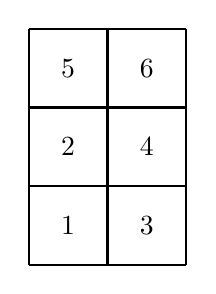
\begin{tikzpicture}[baseline=(current bounding box.center), scale=1, thick]
      \draw (0, 0) grid (2, 3);

      % Row 3
      \node at (0.5, 2.5) {5}; \node at (1.5, 2.5) {6};
      % Row 2 
      \node at (0.5, 1.5) {2}; \node at (1.5, 1.5) {4};
      % Row 1 
      \node at (0.5, 0.5) {1}; \node at (1.5, 0.5) {3};
    \end{tikzpicture}
  \end{subfigure}
  \caption{Rerooting at edge $6$ for $P_3$}
  \label{fig:rerooting-P3}
\end{figure}

We have not yet understood the behavior of the Young tableau when rerooting at non-rerootable edges, which is also an interesting question.

\section{Checking if two prographs' duals are the same triangulation of the sphere}

We use Whitney's 2-Isomorphism Theorem \cite{whitney19922}, checking if the duals are 2-isomorphic.

\section{Partition of the prographs by equivalence classes of dual triangulations for \texorpdfstring{$n=2$}{n=2}}

We illustrate the triangulations by the duals of $P_1$, $P_2$ and $P_3$ in Figure   \ref{fig:prographs-n2-triangulations}. They are all different. The graph $P_2'$ is dual to the same triangulation as $P_2$, and $P_3'$ is dual to the same triangulation as $P_3$ due to symmetry. Thus, there are three equivalence classes of prographs for $n=2$, namely $\{P_1\}$, $\{P_2, P_2'\}$ and $\{P_3, P_3'\}$.

\begin{figure}[ht]
  \centering
  \begin{subfigure}[t]{0.3\textwidth}
    \centering
    \begin{tikzpicture}[baseline=(current bounding box.center), scale=0.6, thick]
      \node[bcircle] (c1) at (0, 0) {};

      \coordinate  (e21) at (-1, 1);
      \coordinate (e22) at (1, 1);

      \node[bsquare] (s31) at (0, 2) {};

      \node[bcircle] (c41) at (0, 4) {};

      \coordinate  (e51) at (-1, 5);
      \coordinate  (e52) at (1, 5);

      \node[bsquare] (s61) at (0, 6) {};

      \node[brhombus, fill=red] (r1) at (0, 1) {};
      \node[brhombus, fill=red] (r3) at (0, 5) {};
      \node[brhombus, fill=red] (r21) at (-2, 3) {};
      \node[brhombus, fill=red] (r22) at (2, 3) {};

      \draw[color=red] (r1) -- (r21)
      (r1) -- (r22)
      (r3) -- (r21)
      (r3) -- (r22)
      (r21) -- (r22);
      \draw[dashed, color=red] (r21) to[out=90, in=90, looseness=1] (r22);

      \draw (0, -0.8)
      edge[->, dashed] (c1);

      \draw (s61)
      edge[dashed] (0, 6.8);

      \draw[dashed] (0, 6.8) to[out=0, in=0, looseness=1] node[right] {} (0, -0.8);

      \draw (c1) -- node[left=0.1cm] {} (e21);
      \draw[-] (e21) -- (s31);
      \draw[-] (s31) -- node[left=0.1cm] {} (c41);
      \draw (c41) -- node[left=0.1cm] {} (e51);
      \draw[-] (e51) -- (s61);

      \draw (c1) -- node[right=0.1cm] {} (e22);
      \draw[-] (e22) -- (s31);

      \draw (c41) -- node[right=0.1cm] {} (e52);
      \draw[-] (e52) -- (s61);
    \end{tikzpicture}
  \end{subfigure}
  \hfill
  \begin{subfigure}[t]{0.3\textwidth}
    \centering
    \begin{tikzpicture}[baseline=(current bounding box.center), scale=0.6, thick]
      \node[bcircle] (c1) at (0, 0) {};

      \coordinate  (e21) at (-2, 2);
      \node[bcircle] (c22) at (2, 2) {};

      \node[bsquare] (s31) at (0, 4) {};
      \coordinate  (e32) at (4, 4);

      \node[bsquare] (s41) at (2, 6) {};

      \node[brhombus, fill=red] (r1) at (0, 2) {};
      \node[brhombus, fill=red] (r21) at (-2, 4) {};
      \node[brhombus, fill=red] (r22) at (2, 4) {};
      \node[brhombus, fill=red] (r23) at (4, 2) {};

      \draw[color=red]
      (r1) -- (r21)
      (r1) -- (r22)
      (r21) -- (r22)
      (r1) -- (r23)
      (r22) -- (r23);

      \draw[dashed, color=red] (r21) to[out=90, in=90, looseness=1] (r23);


      \draw (0, -0.8) edge[-, dashed] (c1);
      \draw (2, 6.8) edge[dashed] (2, 6);
      \draw[dashed] (2, 6.8) to[out=0, in=0, looseness=1.5] node[right] {} (0, -0.8);

      \draw (c1) -- node[left=0.1cm] {} (e21);
      \draw[-] (e21) -- (s31);
      \draw (c1) edge[-] node[right=0.1cm] {} (c22);
      \draw[-] (c22) -- node[left=0.1cm] {} (s31);
      \draw[-] (s31) -- node[left=0.1cm] {} (s41);
      \draw (c22) -- node[right=0.1cm] {} (e32);
      \draw[-] (e32) -- (s41);
    \end{tikzpicture}
  \end{subfigure}\hfill
  \begin{subfigure}[t]{0.3\textwidth}
    \centering
    \begin{tikzpicture}[baseline=(current bounding box.center), scale=0.6, thick]
      \node[bcircle] (c1) at (0, 0) {};

      \node[bcircle] (c21) at (-2, 2) {};
      \coordinate  (e22) at (2, 2);

      \coordinate (e2-51) at (-3, 3);
      \coordinate (e2-52) at (-1, 3);
      \coordinate (e2-53) at (3, 3);

      \node[bsquare] (s31) at (-2, 4) {};

      \node[bsquare] (s41) at (0, 6) {};

      \node[brhombus, fill=red] (r11) at (-4, 3) {};
      \node[brhombus, fill=red] (r12) at (-2, 3) {};
      \node[brhombus, fill=red] (r13) at (0, 3) {};
      \node[brhombus, fill=red] (r14) at (5, 3) {};

      \draw[color=red]
      (r11) -- (r12)
      (r12) -- (r13)
      (r13) -- (r14);

      \draw[color=red] (r11) to[out=90, in=90, looseness=1] (r13);
      \draw[color=red] (r11) to[out=-90, in=-90, looseness=1] (r13);
      \draw[color=red, dashed] (r11) to[out=90, in=90, looseness=1] (r14);

      \draw (0, -0.8) edge[->, dashed] (c1);
      \draw (0, 6.8) edge[dashed] (0, 6);
      \draw[dashed] (0, 6.8) to[out=0, in=0, looseness=1.5] node[right] {} (0, -0.8);

      \draw (c1) edge[-] node[left=0.1cm] {} (c21);
      \draw (c21) -- node[left=0.1cm] {} (e2-51)
      (e2-51) edge[-] (s31);
      \draw (c21) -- node[right=0.1cm] {} (e2-52)
      (e2-52) edge[-] (s31);
      \draw (c1) -- node[right=0.1cm] {} (e2-53)
      (e2-53) edge[-] (s41);
      \draw (s31) edge[-] node[left=0.1cm] {} (s41);
    \end{tikzpicture}
  \end{subfigure}

  \caption{The triangulation of the sphere corresponding to the dual of each size-$2$ prograph drawn in red. We omitted the direction and labels for visibility.}
  \label{fig:prographs-n2-triangulations}
\end{figure}